\section{Introduction}

End user programmers' develop by interleaving opportunistic information foraging with writing code~\cite{brandt_two_2009}~\cite{brandt_example-centric_2010}.
As online coverage of common APIs grows~\cite{parnin_measuring_2011}, programmers increasingly use \emph{crowd documentation} like StackOverflow and blog postings.
Such documentation can be written by coders who lack interest or expertise in writing usable documentation.
Both experienced programmers~\cite{duala-ekoko_asking_2012} and end-user programmers~\cite{dorn_lost_2013}\cite{dorn_learning_2010}\cite{rosson_everyday_2004} struggle to leverage web documentation to solve programming problems.
\andrew{Check \cite{dorn_learning_2010}\cite{rosson_everyday_2004} are relevant.}

Decades of research on technical communication provide best practices for writing usable documentation.
For learning how to use software, \emph{minimalist instruction}~\cite{carroll_nurnberg_1990} recommends enabling users to start immediatedly on realistic tasks, reducing the amount of reading and other passive activity, and supporting error recognition and recovery.
Farkas introduces \emph{layered documentation} as an extension to minimalist instruction that enables users from different backgrounds to benefit from the same documents by providing optional \emph{backup information} for tasks like error recognition and correction~\cite{farkas_layering_1998}.

Instructions for web scraping code may assumes a reader has some \emph{base competencies} in Python, callbacks, threads, and micro-languages like CSS selectors, regular expressions.
Given the \emph{diverse backgrounds of both the audience and authors}, it is impractical for the author to introduce all these base competencies in detail.
As a result, today's Q\&A's and blogs lack scaffolding for readers seeking clarification on unfamiliar or complex syntax.

To enable this scaffolded documentation, we propose \emph{\Glspl{name}}: on-demand, context-relevant descriptions of programming languages, commands and libraries that can run on arbitrary code found anywhere.
\andrew{Still not clear if \glspl{name} are explainers or explanations.}
Such explanations can describe syntax for languages like CSS selectors and regular expressions.
A \gls{name} for a language or command is programmed in several hundred lines of code to both \emph{parse} and \emph{explain} arbitrary input syntax.
They can be integrated as bookmarklets into a programmer's browser to provide just-in-time explanations of a language, command or API anywhere on the web.
We demonstrate how they can be used to generate text descriptions at multiple levels of detail.



Our contributions in this paper are as follows.
First, we demonstrate of a need for micro-explanations by showing underexplained, assumed \emph{base competencies} in popular StackOverflow answers.
Second, we propose an architecture for \glspl{name}, automatic natural language generators for describing programming languages, commands and APIs.
Third, we demonstrate the technical effort required to build \glspl{name} by building them for CSS selectors, command lines, and regular expressions.
Finally, we evaluate their utility through an informal in-lab study where we have users perform transfer tasks with tutorials augmented with \gls{name}-generated explanations.

\begin{figure}[!t]
\centering{
    \subfigure[Text augmentation explaining a CSS selector]{
        \framebox{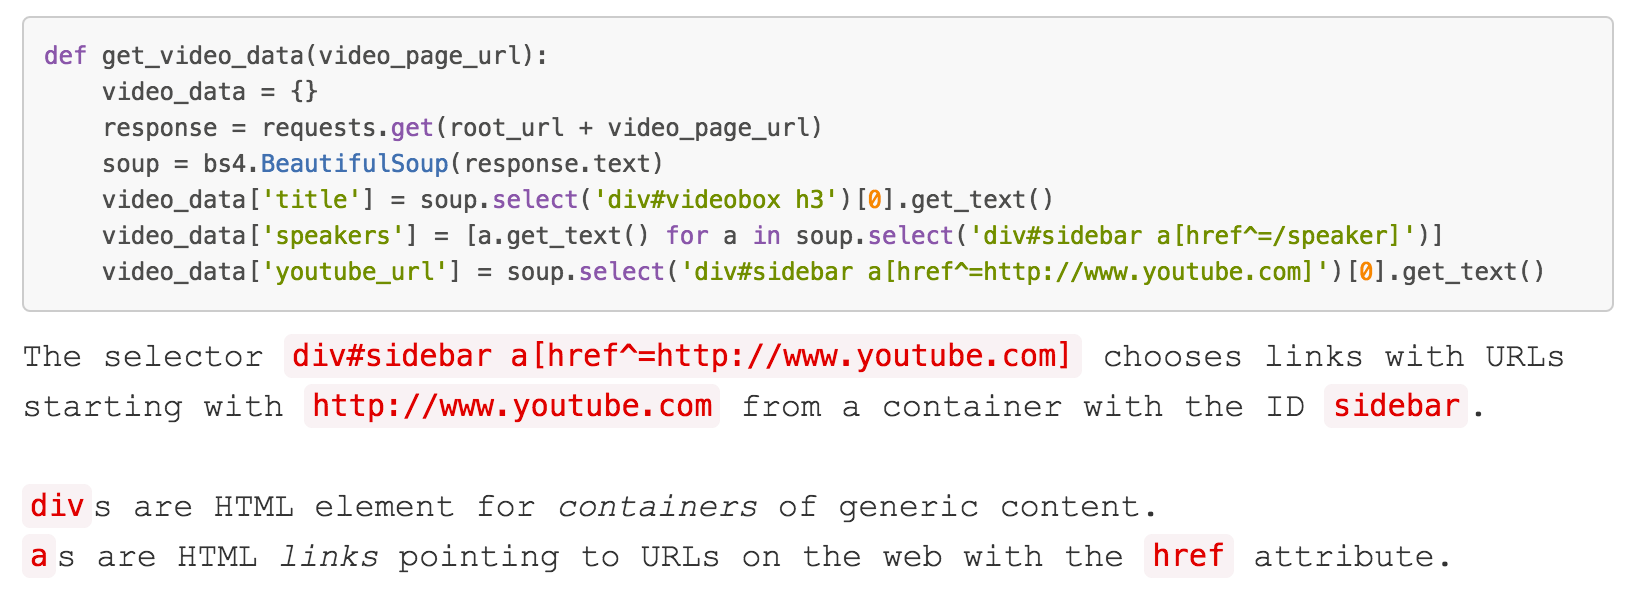
\includegraphics[width=.4\textwidth]{figures/css_explanation}}
        \label{fig:css_explanation}
    }
}
\label{fig:tutorons}
\caption{Automatic, context-relevant textual and visual explanations of code generated by descriptive \glspl{name}.}
\end{figure}
